\chapter{Discussion}

\todo{What was improved and why? DISCUSS OVERALL! Talk about why we got new parts for V2, limitations of current apparatus and future directions}

% why do we prefer spark ignition
This project was started on the heels of \textcite{duplayArgonLaserPlasmaThruster2024a}, with the V1 test section using wire initiation during summer 2023. Spark initiation is preferred for a few reasons. First, there would be no solid object blocking the beam path. This would allow the power meter to measure the energy that was not absorbed by the plasma, which is the first efficiency considered in\todo{Link to intro?}. Second, replacing the target wire is a time consuming process that was conducted every 1-3 shots, requiring the test section to be re-pressurized. Indeed, spark initiation would allow a much higher shot rate. Third, when conducting flowing experiments, the wire could be moved out of the focus by the flowing argon. Finally, the wire prevents the downstream propagation of the plasma by being physically in the way.

With V1, spark initiation was first attempted with an initiation plug that could fit into a single port \todo{photo}. The electrodes were side by side. However, the spark was created at a different height every time between the parallel electrodes. Using opposing electrodes would ensure that their tips were the closest point to each other, greatly increasing spatial repeatability of the spark and enabling the electrode gap length to be easily adjusted. Opposing ports were drilled into the bottom of the V1 apparatus to fit an electrode through the top and one through the bottom \todo{photo of electrode plugs}.

\begin{figure}[!ht]
    \centering
    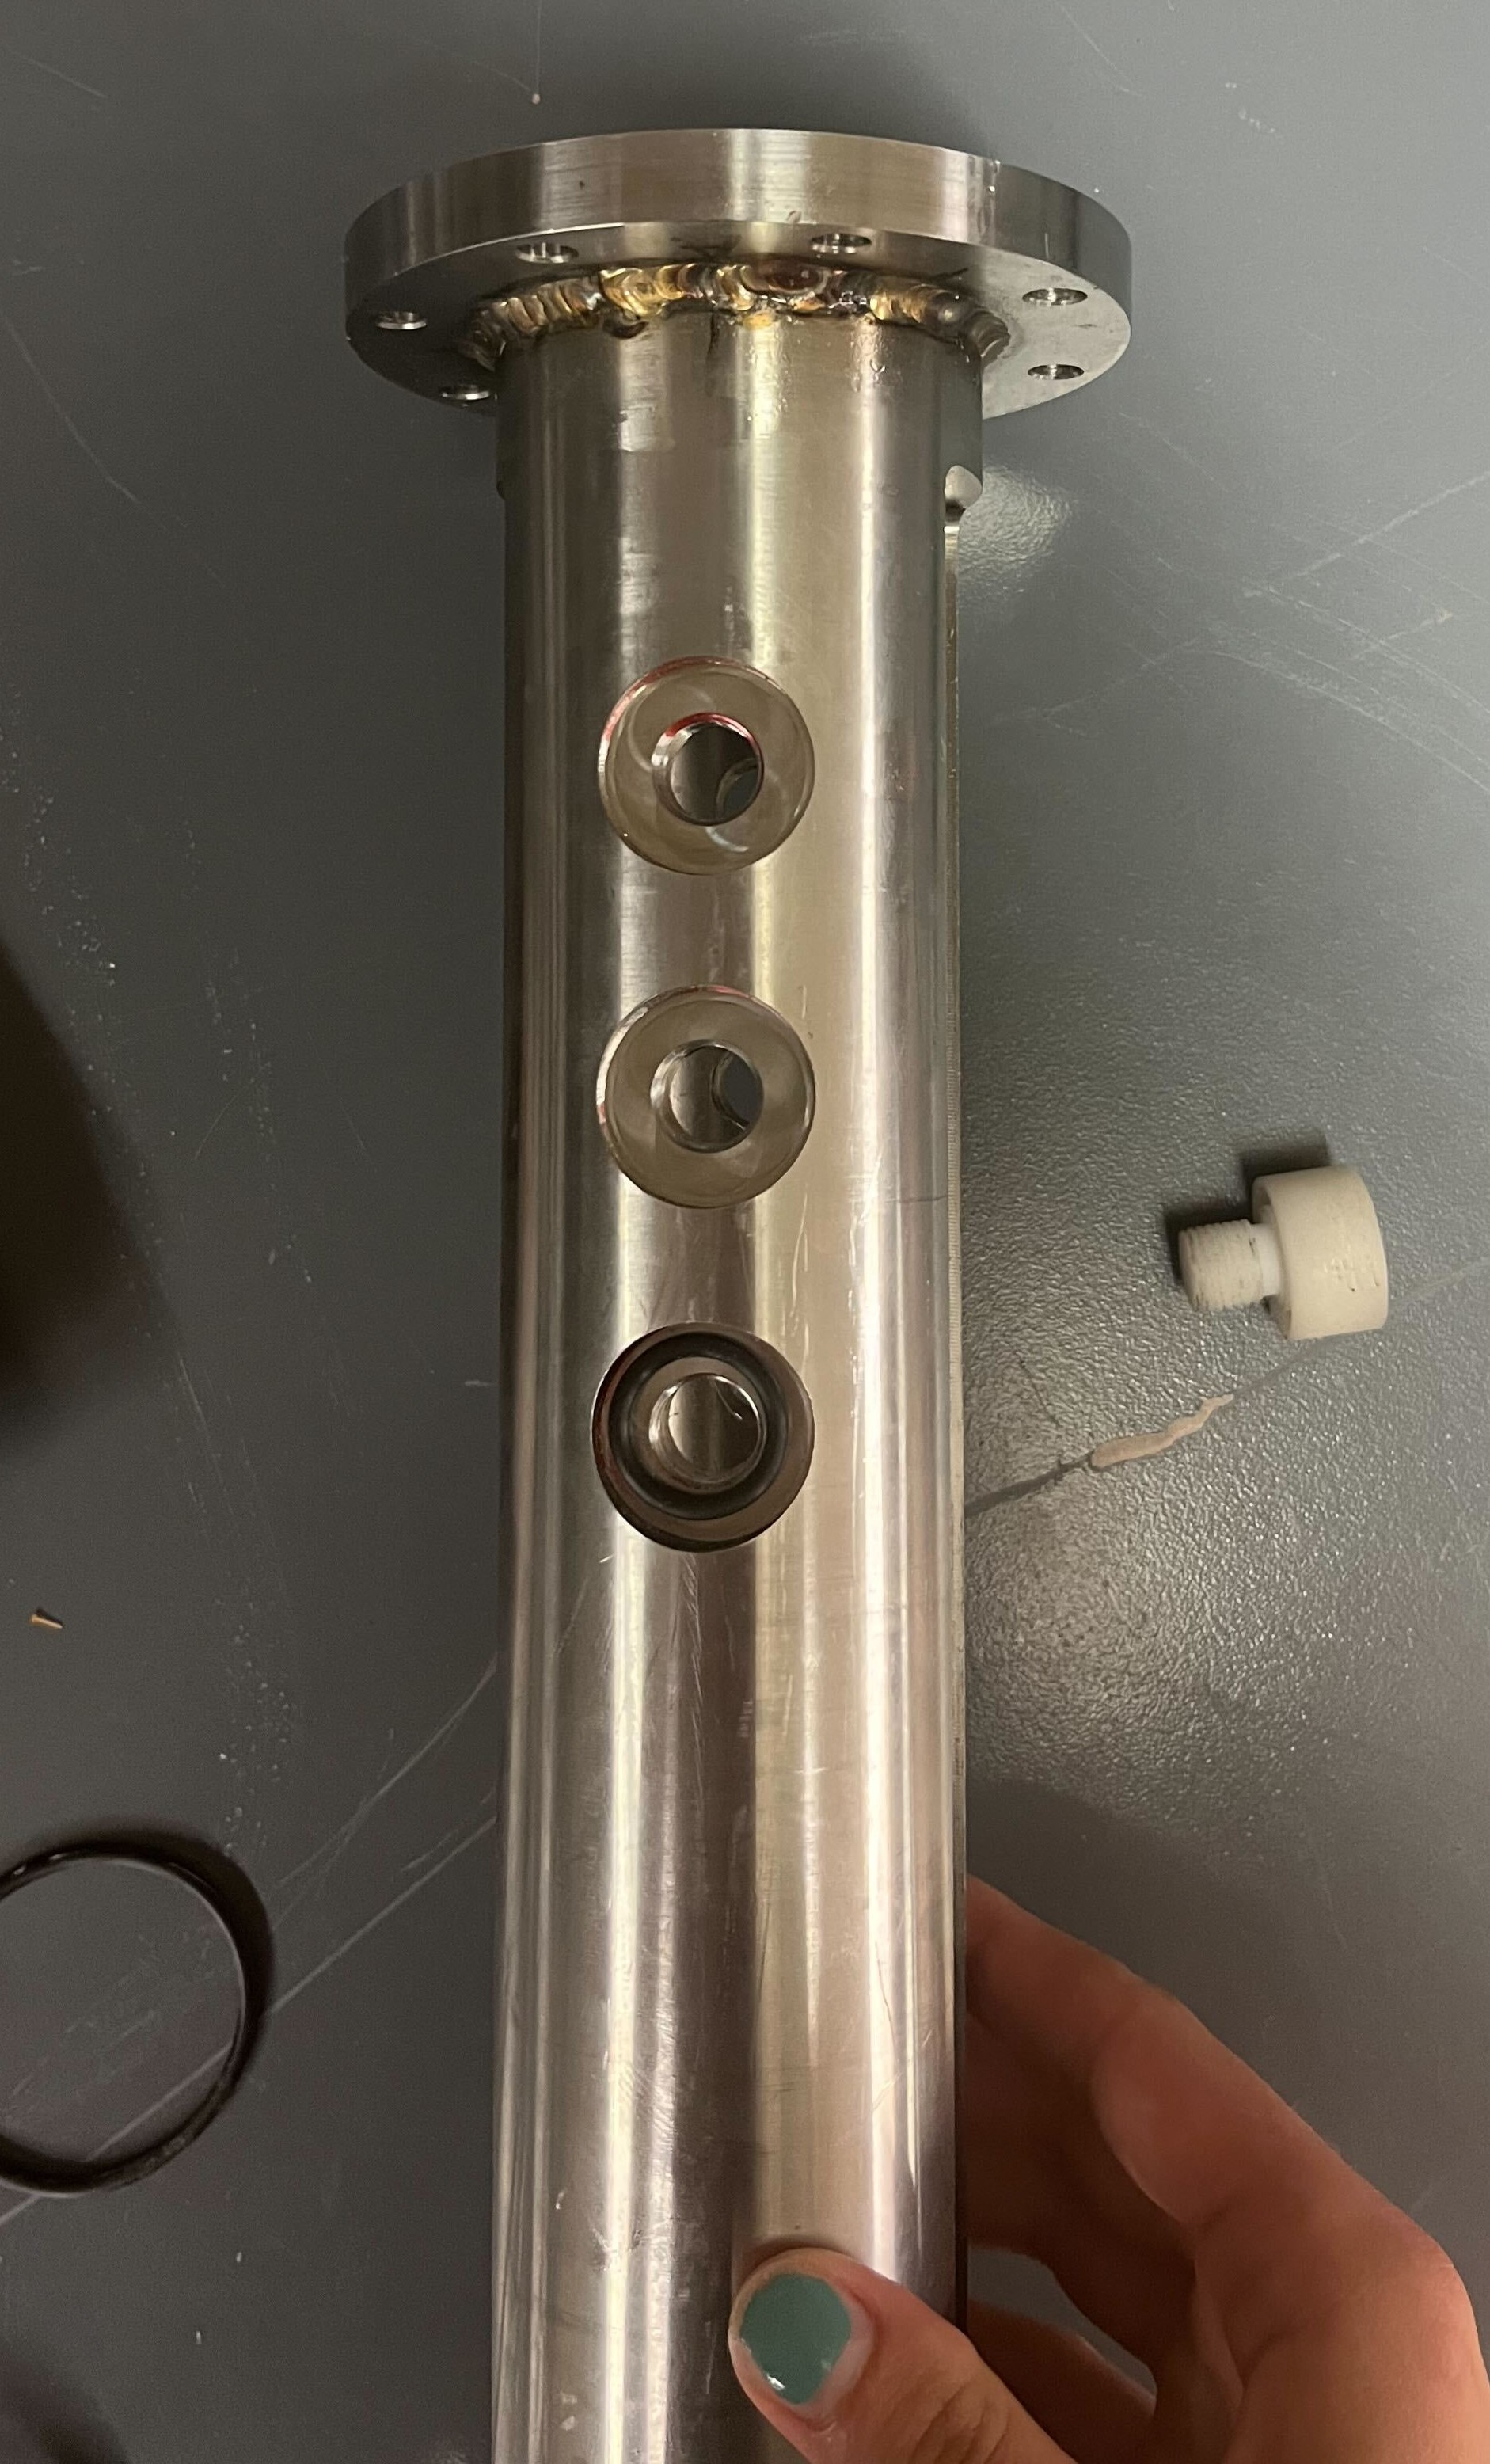
\includegraphics[width=0.5\textwidth]{assets/5 discussion/Bottom ports machined.jpg}
    \caption{V1 with newly machined opposing bottom ports}
\end{figure}

%% % In addition to this, the synchronization of the spark and the laser was found to be lacking.

% Coil burnout
Another critical issue was that of coil burnout. 5 coils were damaged to the point that they could no longer create a strong enough spark across the spark gap. A contributing factor could have been the poor electrode retention of the Ultra-Torr fittings, as \qty{20}{bar} of gas could visibly push the electrodes away \qtyrange{1}{2}{mm}. An increase in the spark gap increases its resistance, putting a higher load on the coil. Another concern was electromagnetic interference between the coil and its power supply. Originally in the same box, the \qty{10}{A} current-limited power supply and the smart coil were placed in separate electrical boxes. Quad shielded coaxial cable was used between the coil, and it's controlling delay generator as an additional precaution. 

% TALK ABOUT TIMING?

% V1 spark initiation! + Why was V2 designed?
With these problems solved, reliable spark initiation of LSP was achieved in V1 \todo{When?}. 

However, this test section was made of steel, creating too much friction on its rails during thrust tests. This was mitigated in part by a rope system mentioned in \textcite{duplayArgonLaserPlasmaThruster2024a}, but was not found to be repeatable. Having the LSP heat a smaller internal volume than the \qty{0.38}{L} of V1 was also desirable, as a greater effect on internal pressure and thrust would be seen.

Critically, rubber seals were exposed to the laser path during continuous (CW) lasing with a lower focal length lens (picture), severely burning them in the only CW test conducted. A shorter test section designed for a \qty{100}{mm} focal length lens would allow the beam to pass through without hitting the sides of the test section. A purpose-built test section, named V2, was therefore designed over the course of two semesters. 

% Got V2 from capstone team
The achievement of consistent spark initiation with V1 coincided with the arrival of the V2 test section parts in late April. Static pressure testing of V2 up to \qty{75}{bar} for \qty{25}{minutes} was completed successfully. However, the off-the-shelf \qty{44}{kV} wire originally intended to be used as the electrodes burst during pressure tests. An electrode redesign was therefore necessary. Molded dielectric epoxy (Stycast ES 1001 [LINK to website]) around an industrial sewing needle core was chosen, as it was economical and the outer diameter of the electrodes could be precisely controlled by sanding the surface of the set epoxy. Molds were 3d printed and Mann Ease Release\texttrademark 300 was applied to all their inside surfaces.

\begin{figure}[!ht]
    \centering
    \begin{subfigure}[t]{0.30\textwidth}
        \centering
        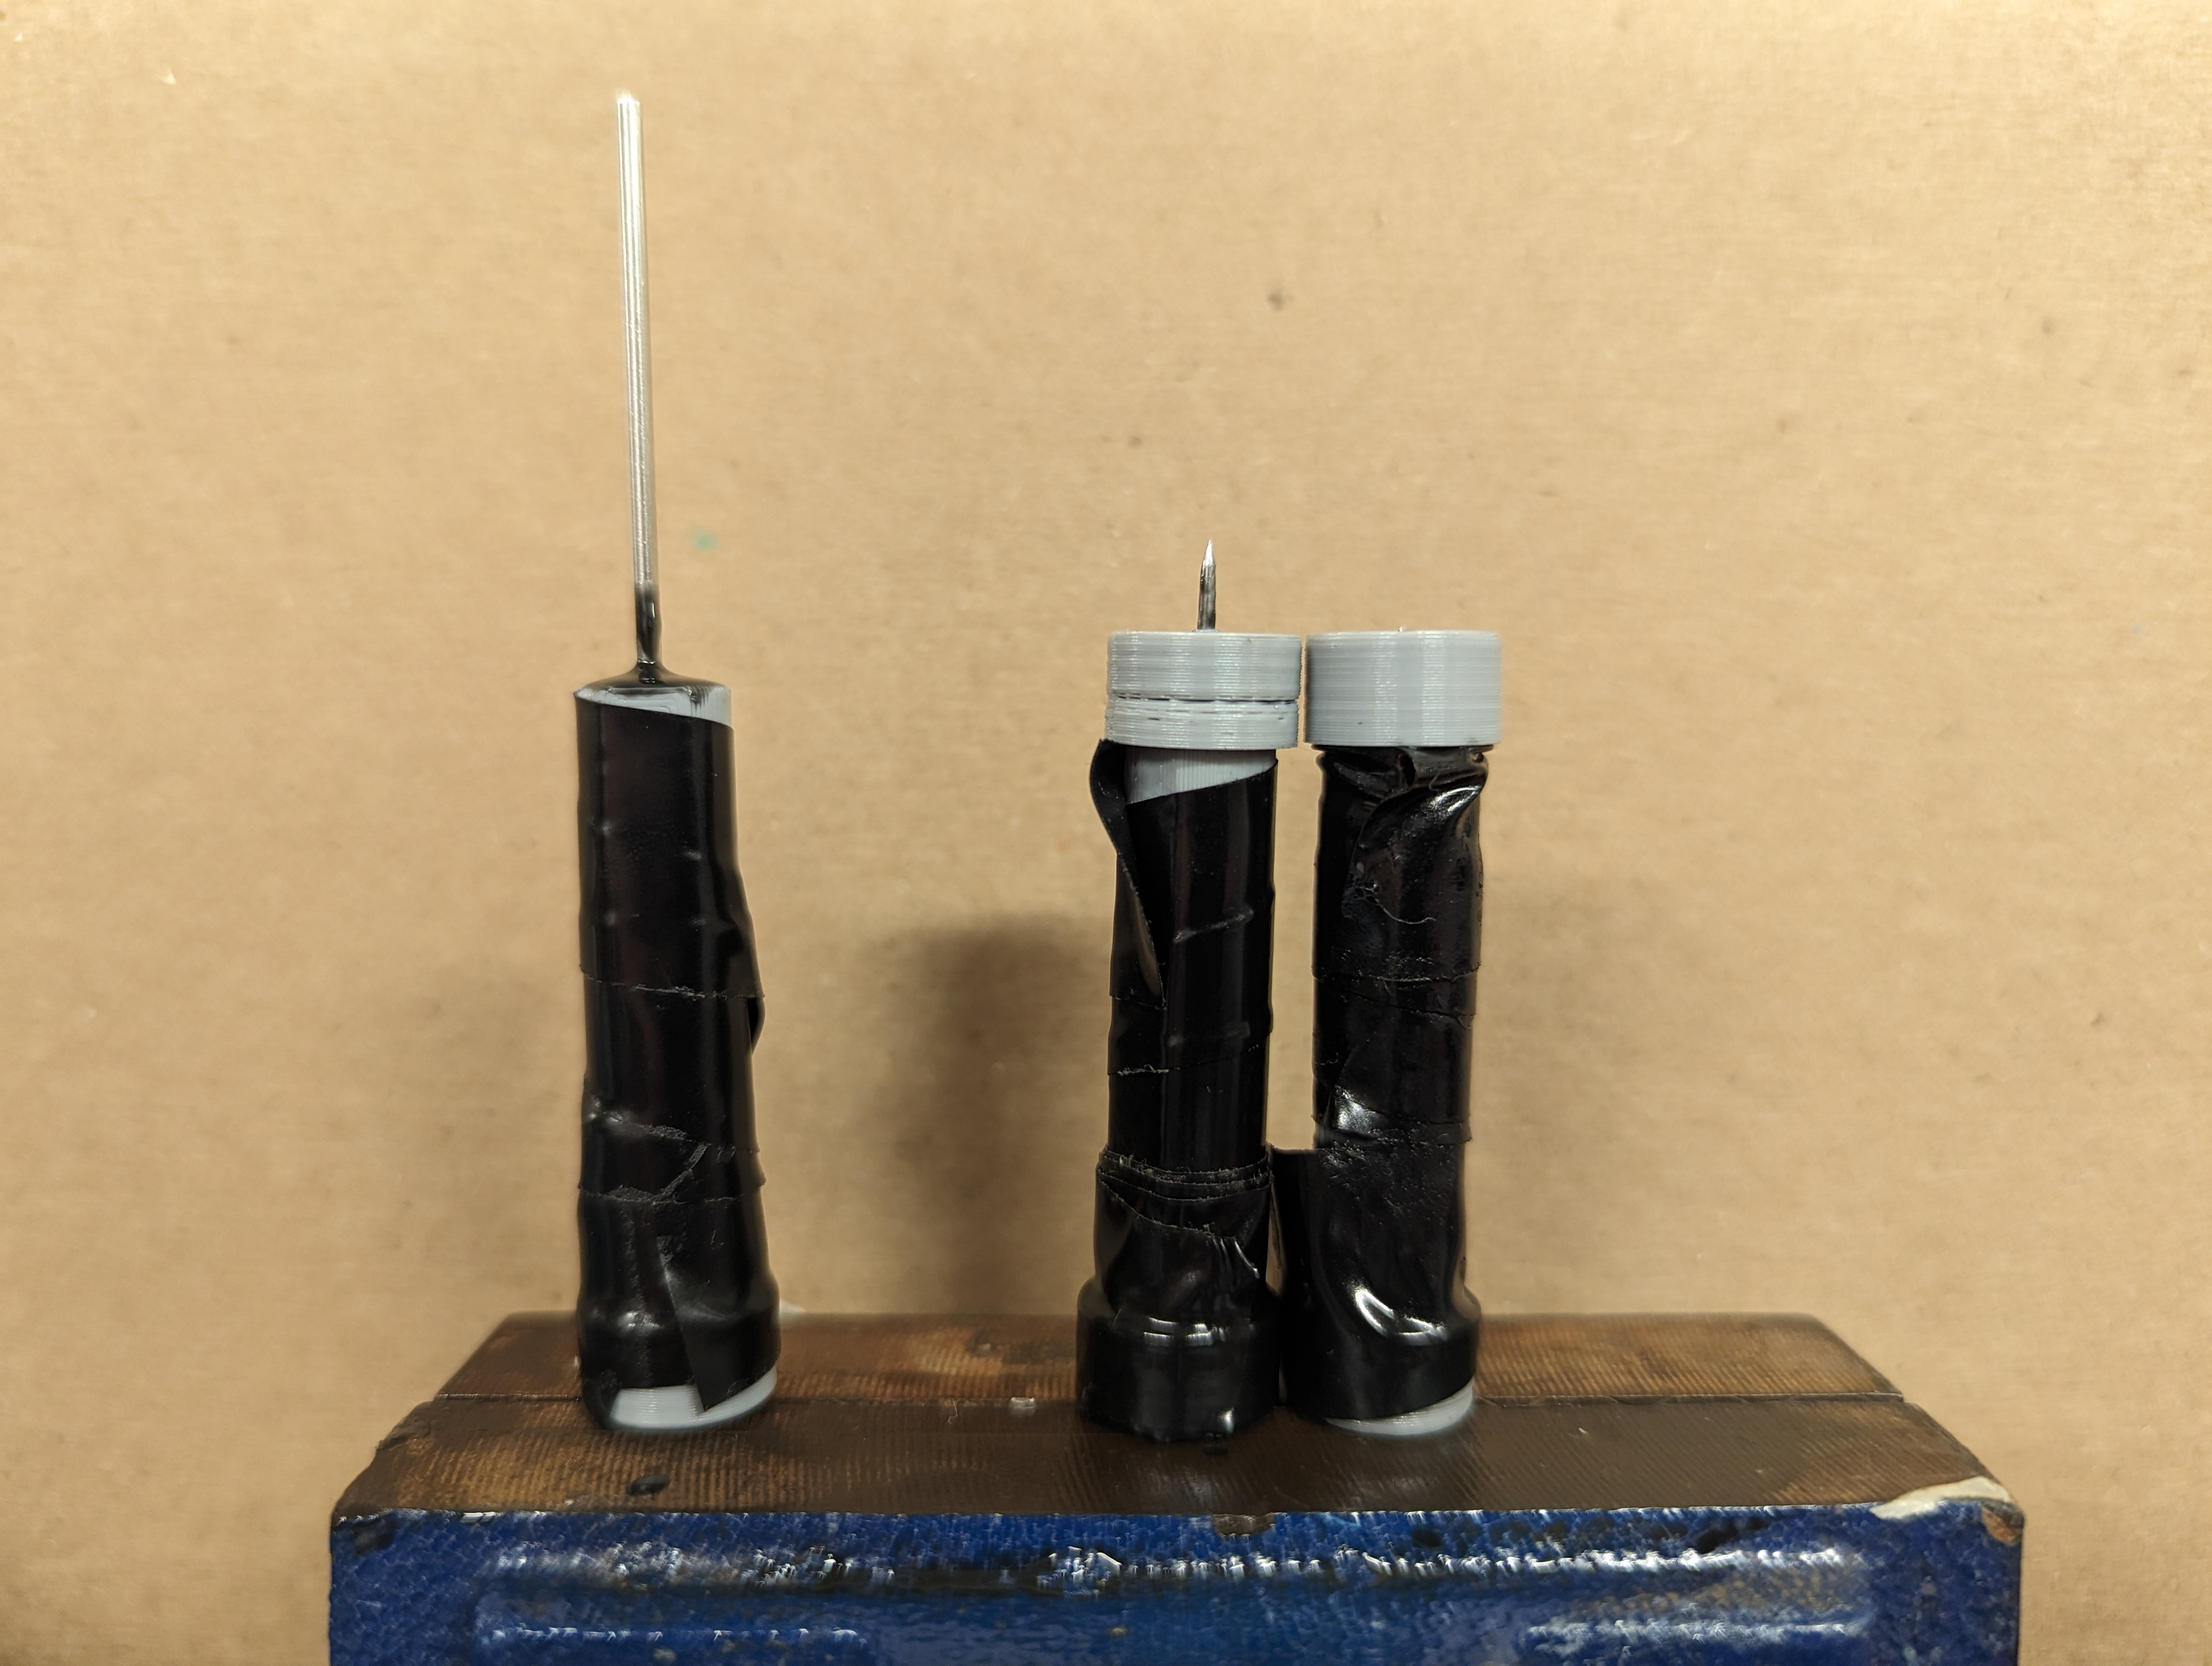
\includegraphics[width=\textwidth]{assets/3 design/Molds.jpg}
        \caption{Molds with steel needle core in place}
    \end{subfigure}
    \hfill
    \begin{subfigure}[t]{0.30\textwidth}
        \centering
        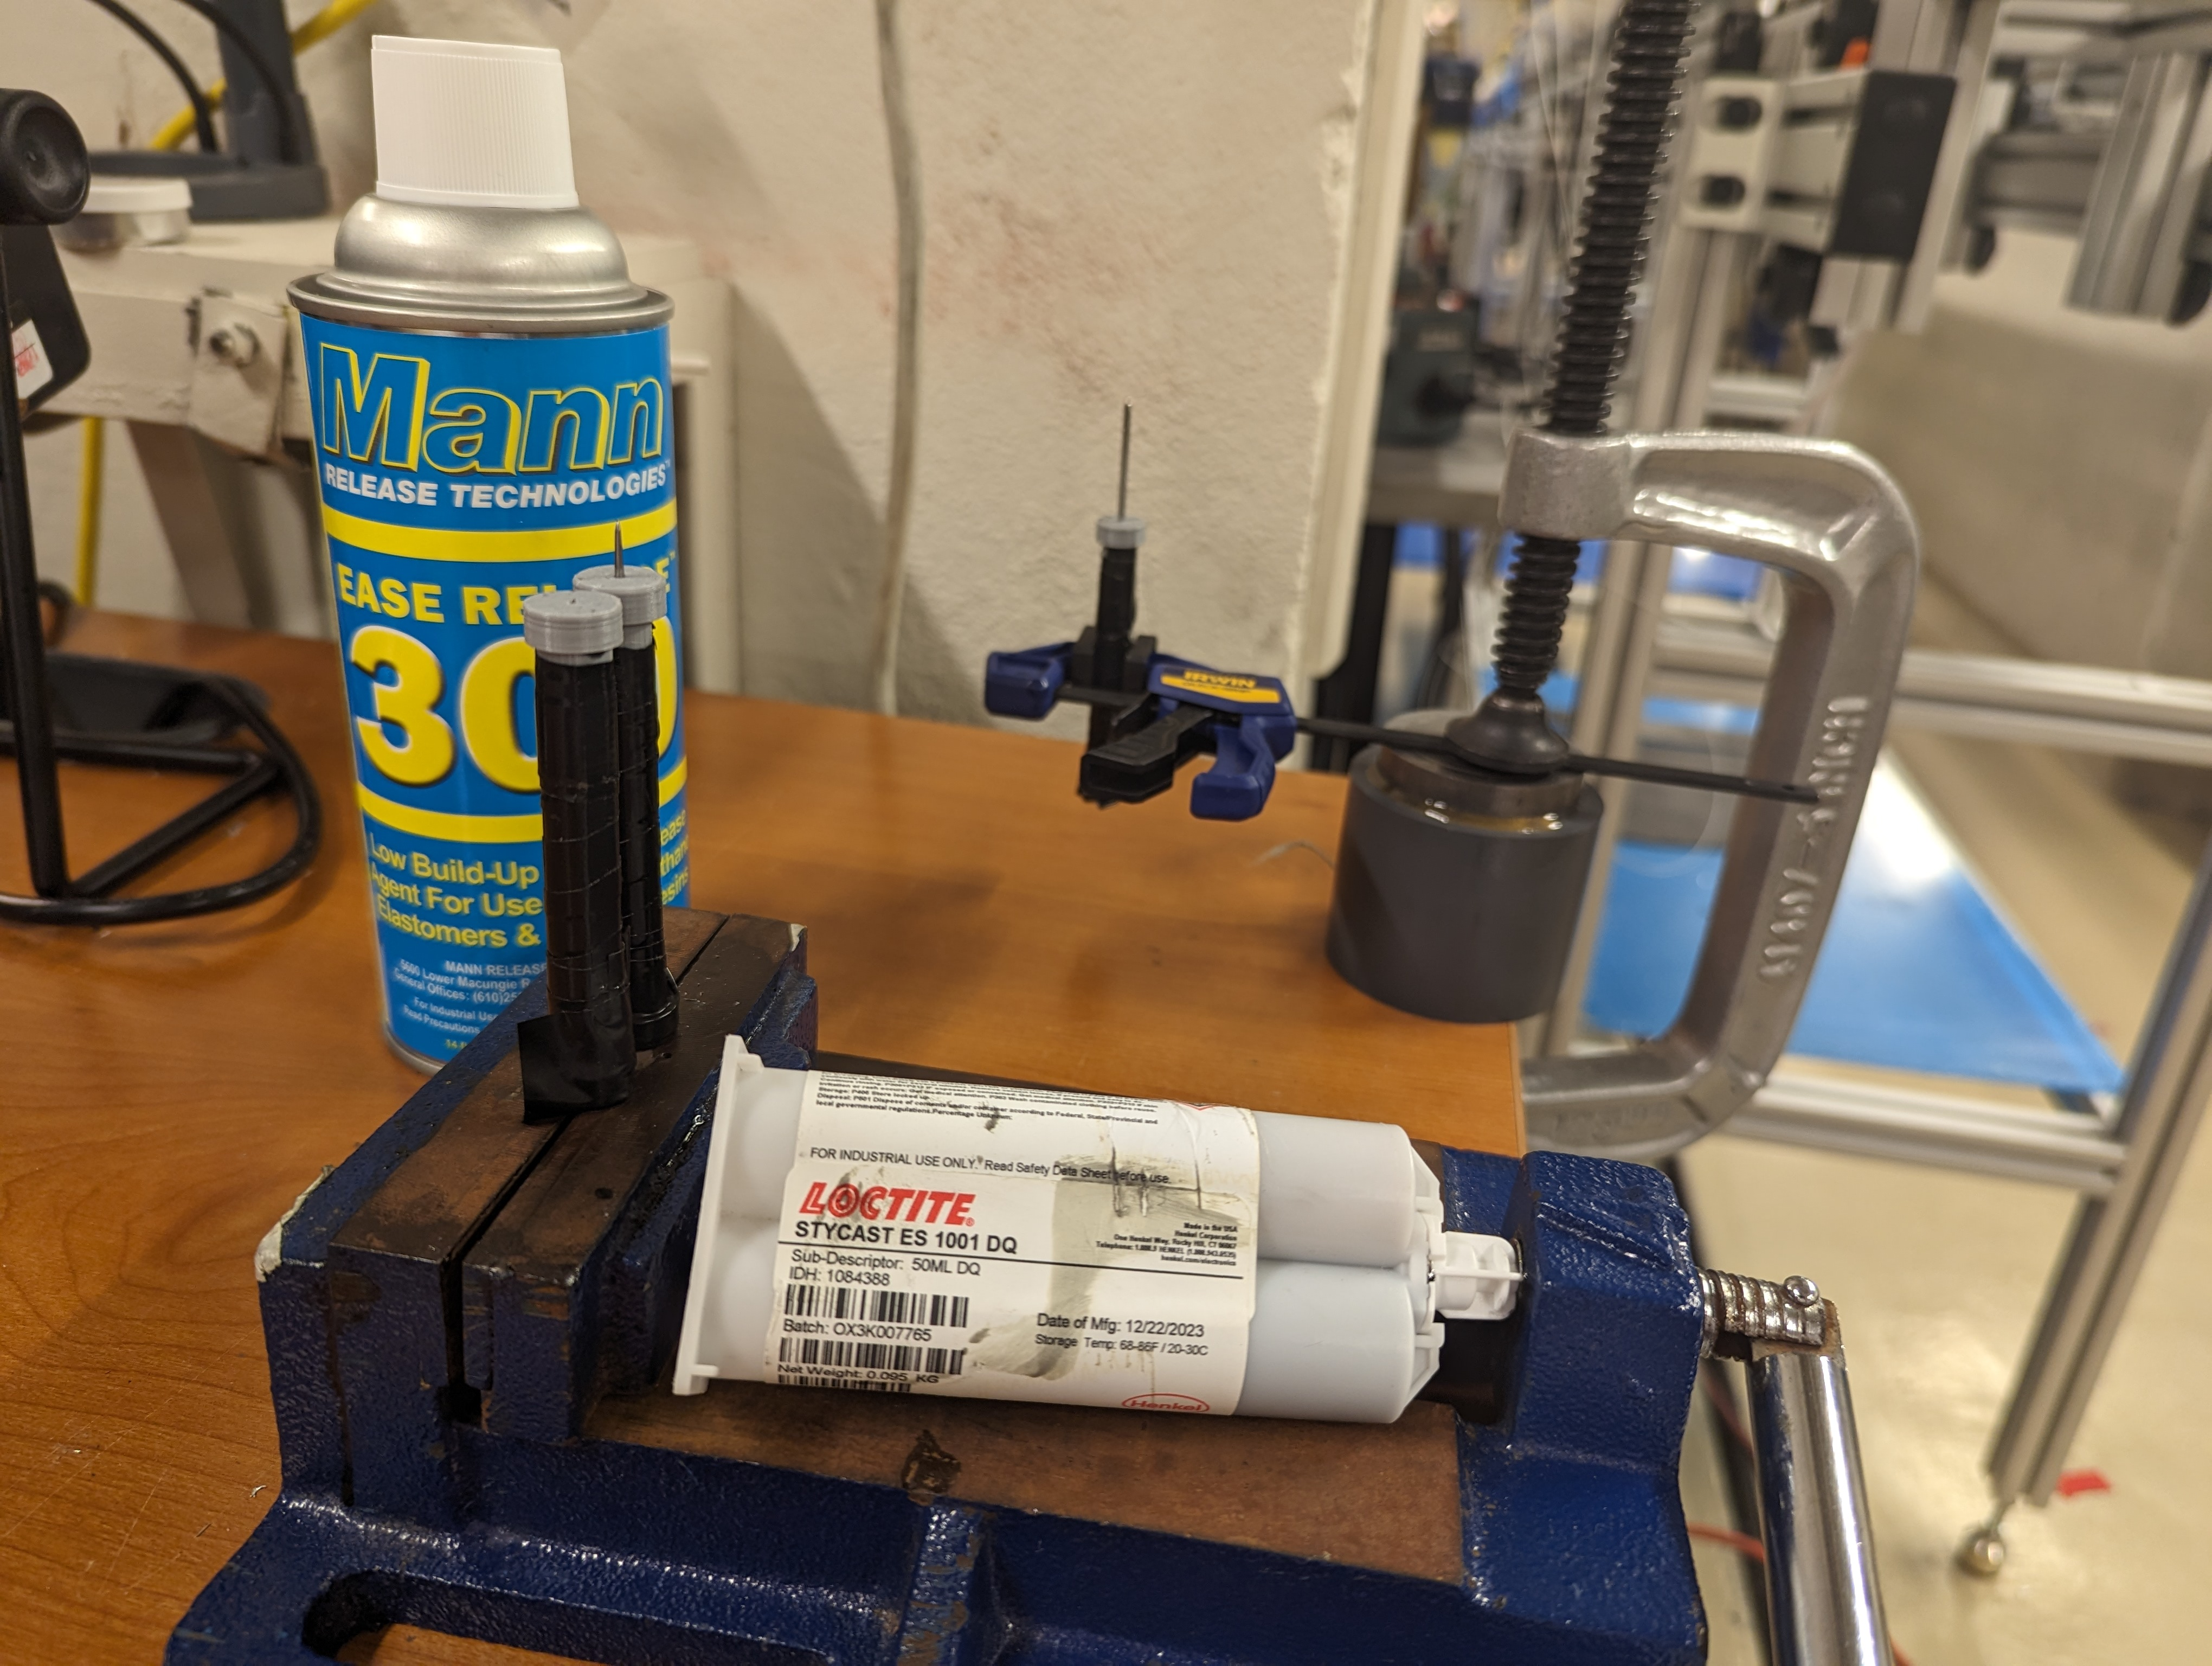
\includegraphics[width=\textwidth]{assets/3 design/Mold process.jpg}
        \caption{Molding process}
    \end{subfigure}
    \hfill
    \begin{subfigure}[t]{0.30\textwidth}
        \centering
        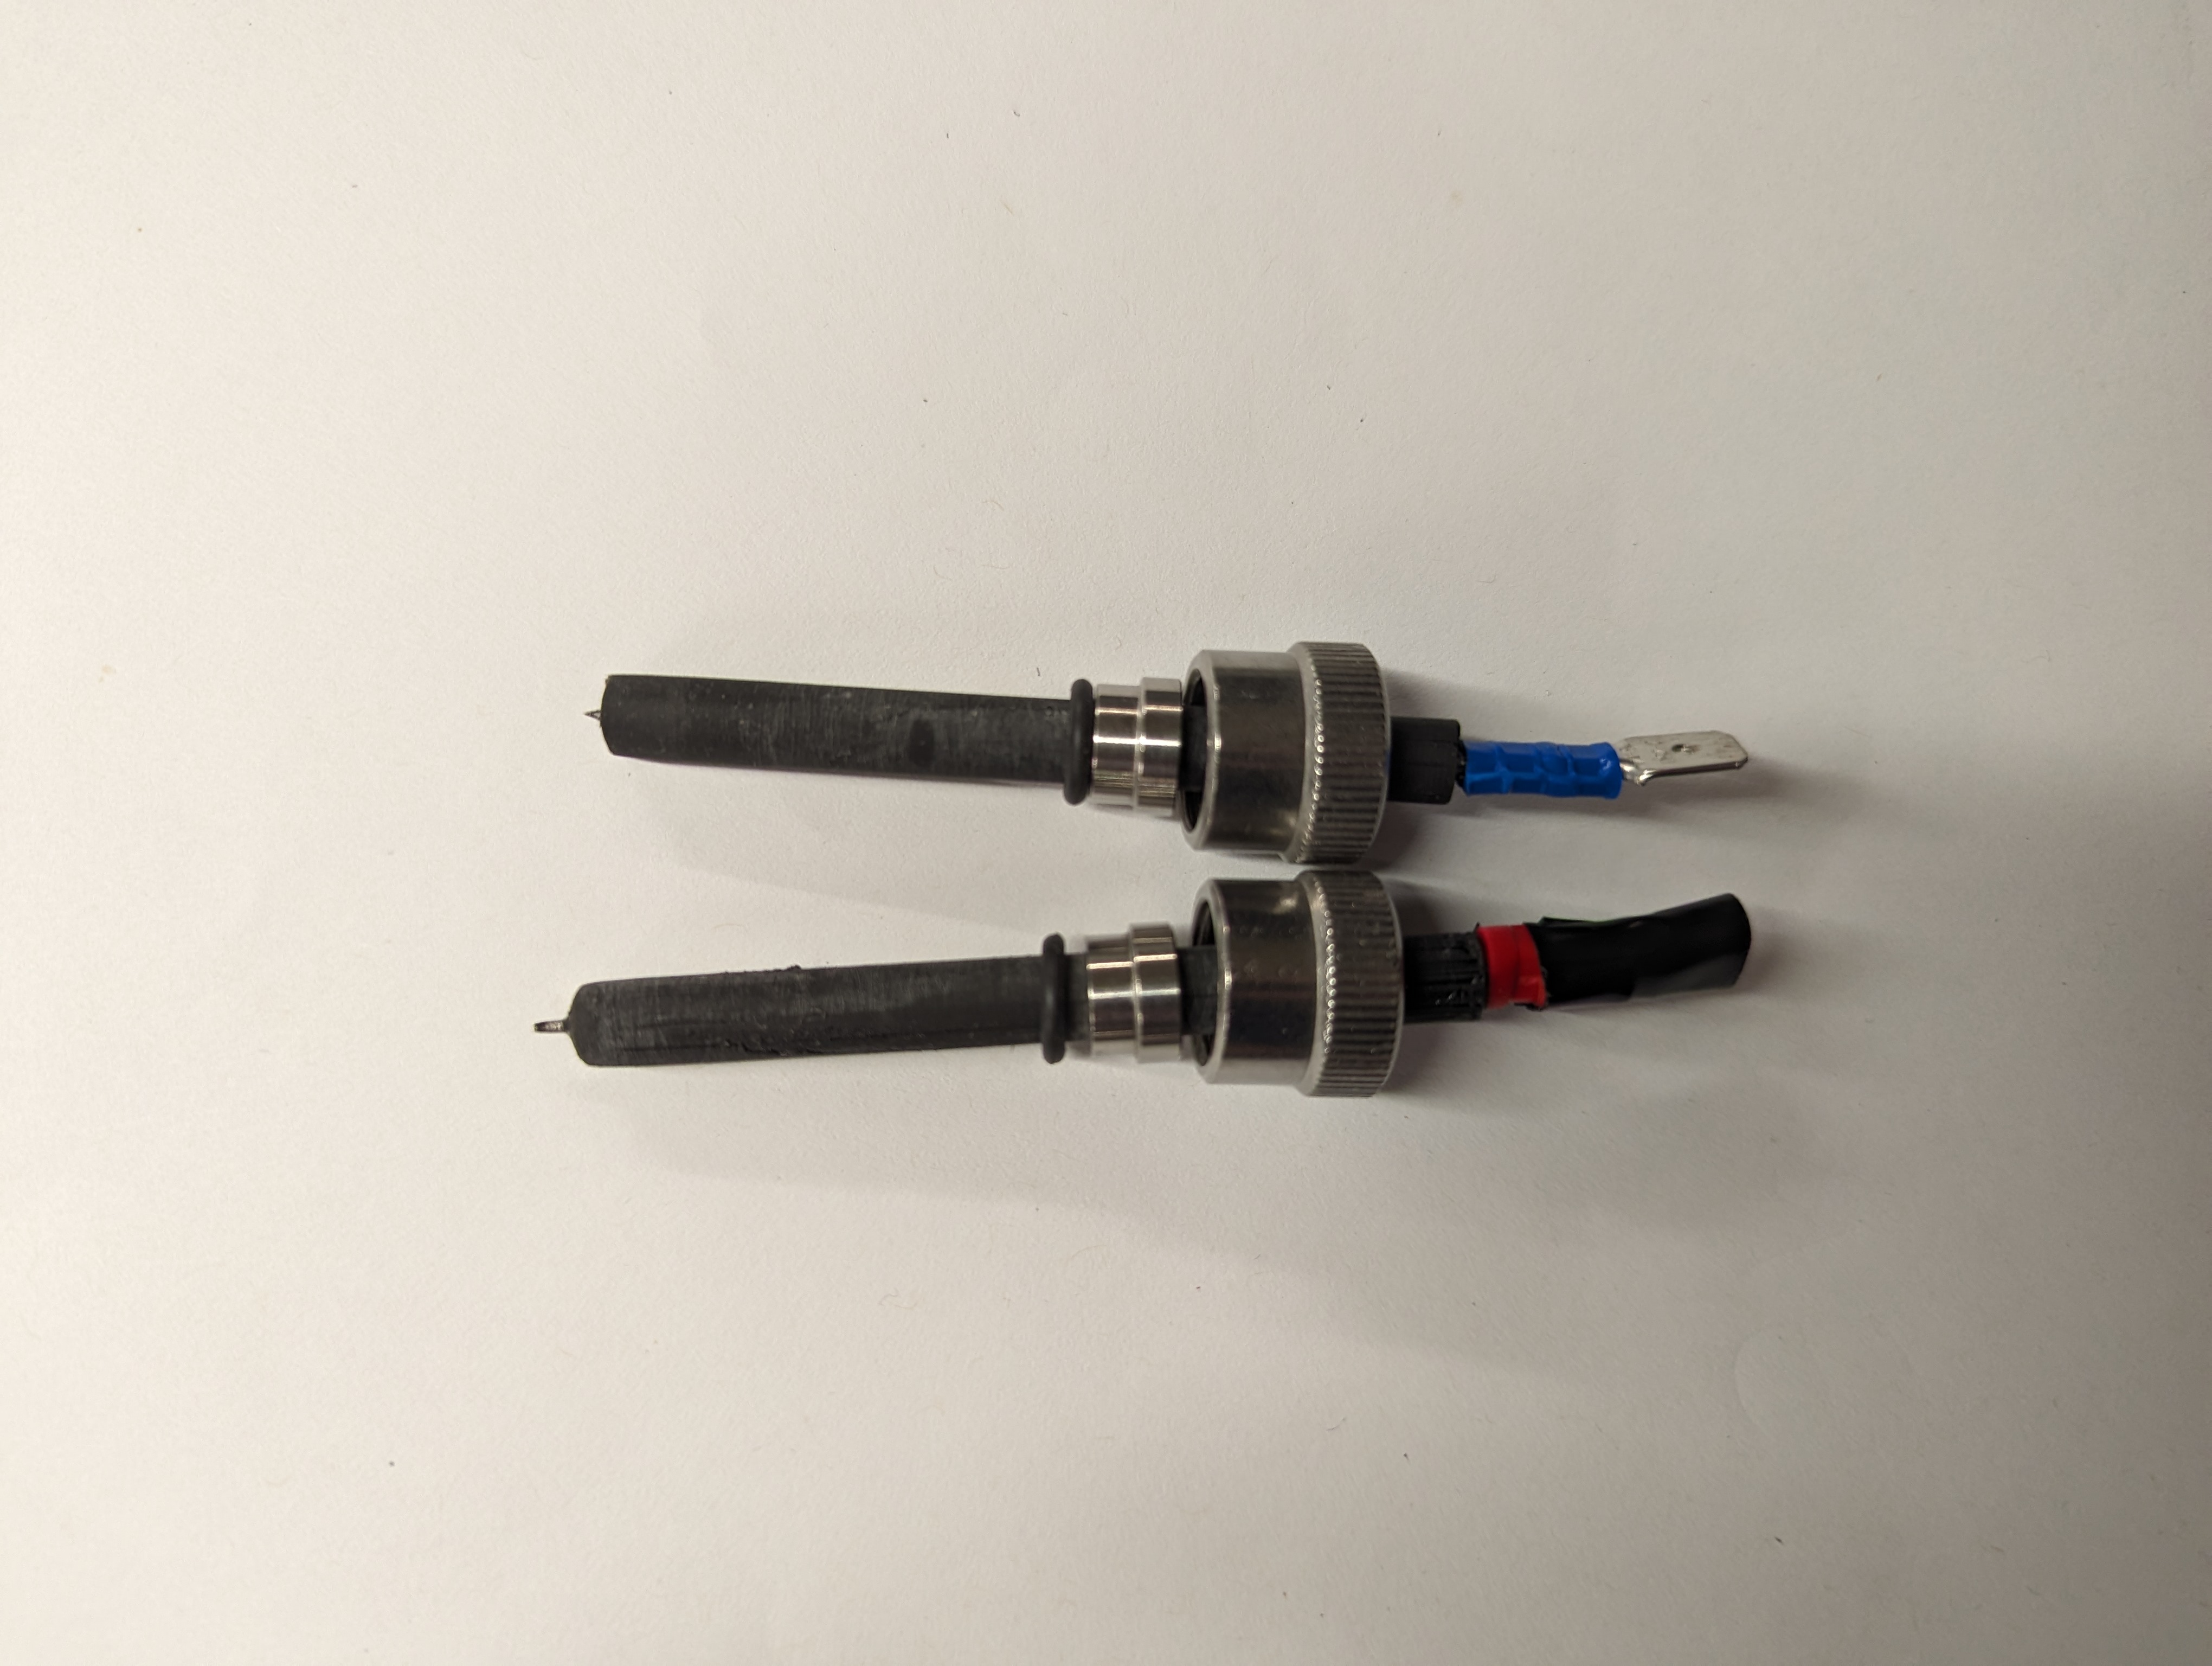
\includegraphics[width=\textwidth]{assets/3 design/V2 electrodes.jpg}
        \caption{Assembled electrodes with Ultra-Torr cap and electrical connectors}
        \label{fig:Assembled electrode}
    \end{subfigure}

    \caption{Electrode manufacturing process}
\end{figure}

The electrodes were then sanded down to fit tightly into Ultra-Torr vacuum connectors [link to swagelok and part number]. Although these connectors were not designed for high pressure, previous experience has shown that they are appropriate up to about \qty{20}{bar} of internal pressure if tightened enough.

The result is presented in \autoref{fig:Assembled electrode}.

Once installed in the V2 thruster, the electrodes were pushed into contact with each other and the Ultra-Torr connectors tightened. Statically pressurizing V2 to \qty{20}{bar} was enough to slightly separate the electrodes from one another. \todo{Put some of this in design section}

\section*{LOTS OF TIME AND THINGS HAPPEN THEN...}


% OLD DISCUSSION
\section*{AFTER THIS IS OLD DISCUSSION}

\section{Static LSP validation}

    \subsection{Improving V2's static LSP configuration}

        [Flat plate -> interim solution aluminum paper, then steel cylinder but can't align.-> needed window, damaged window -> designed window with extension \todo{validate extension}]

        % flat plate with aluminum damage
        \begin{figure}[!ht]
            \centering
            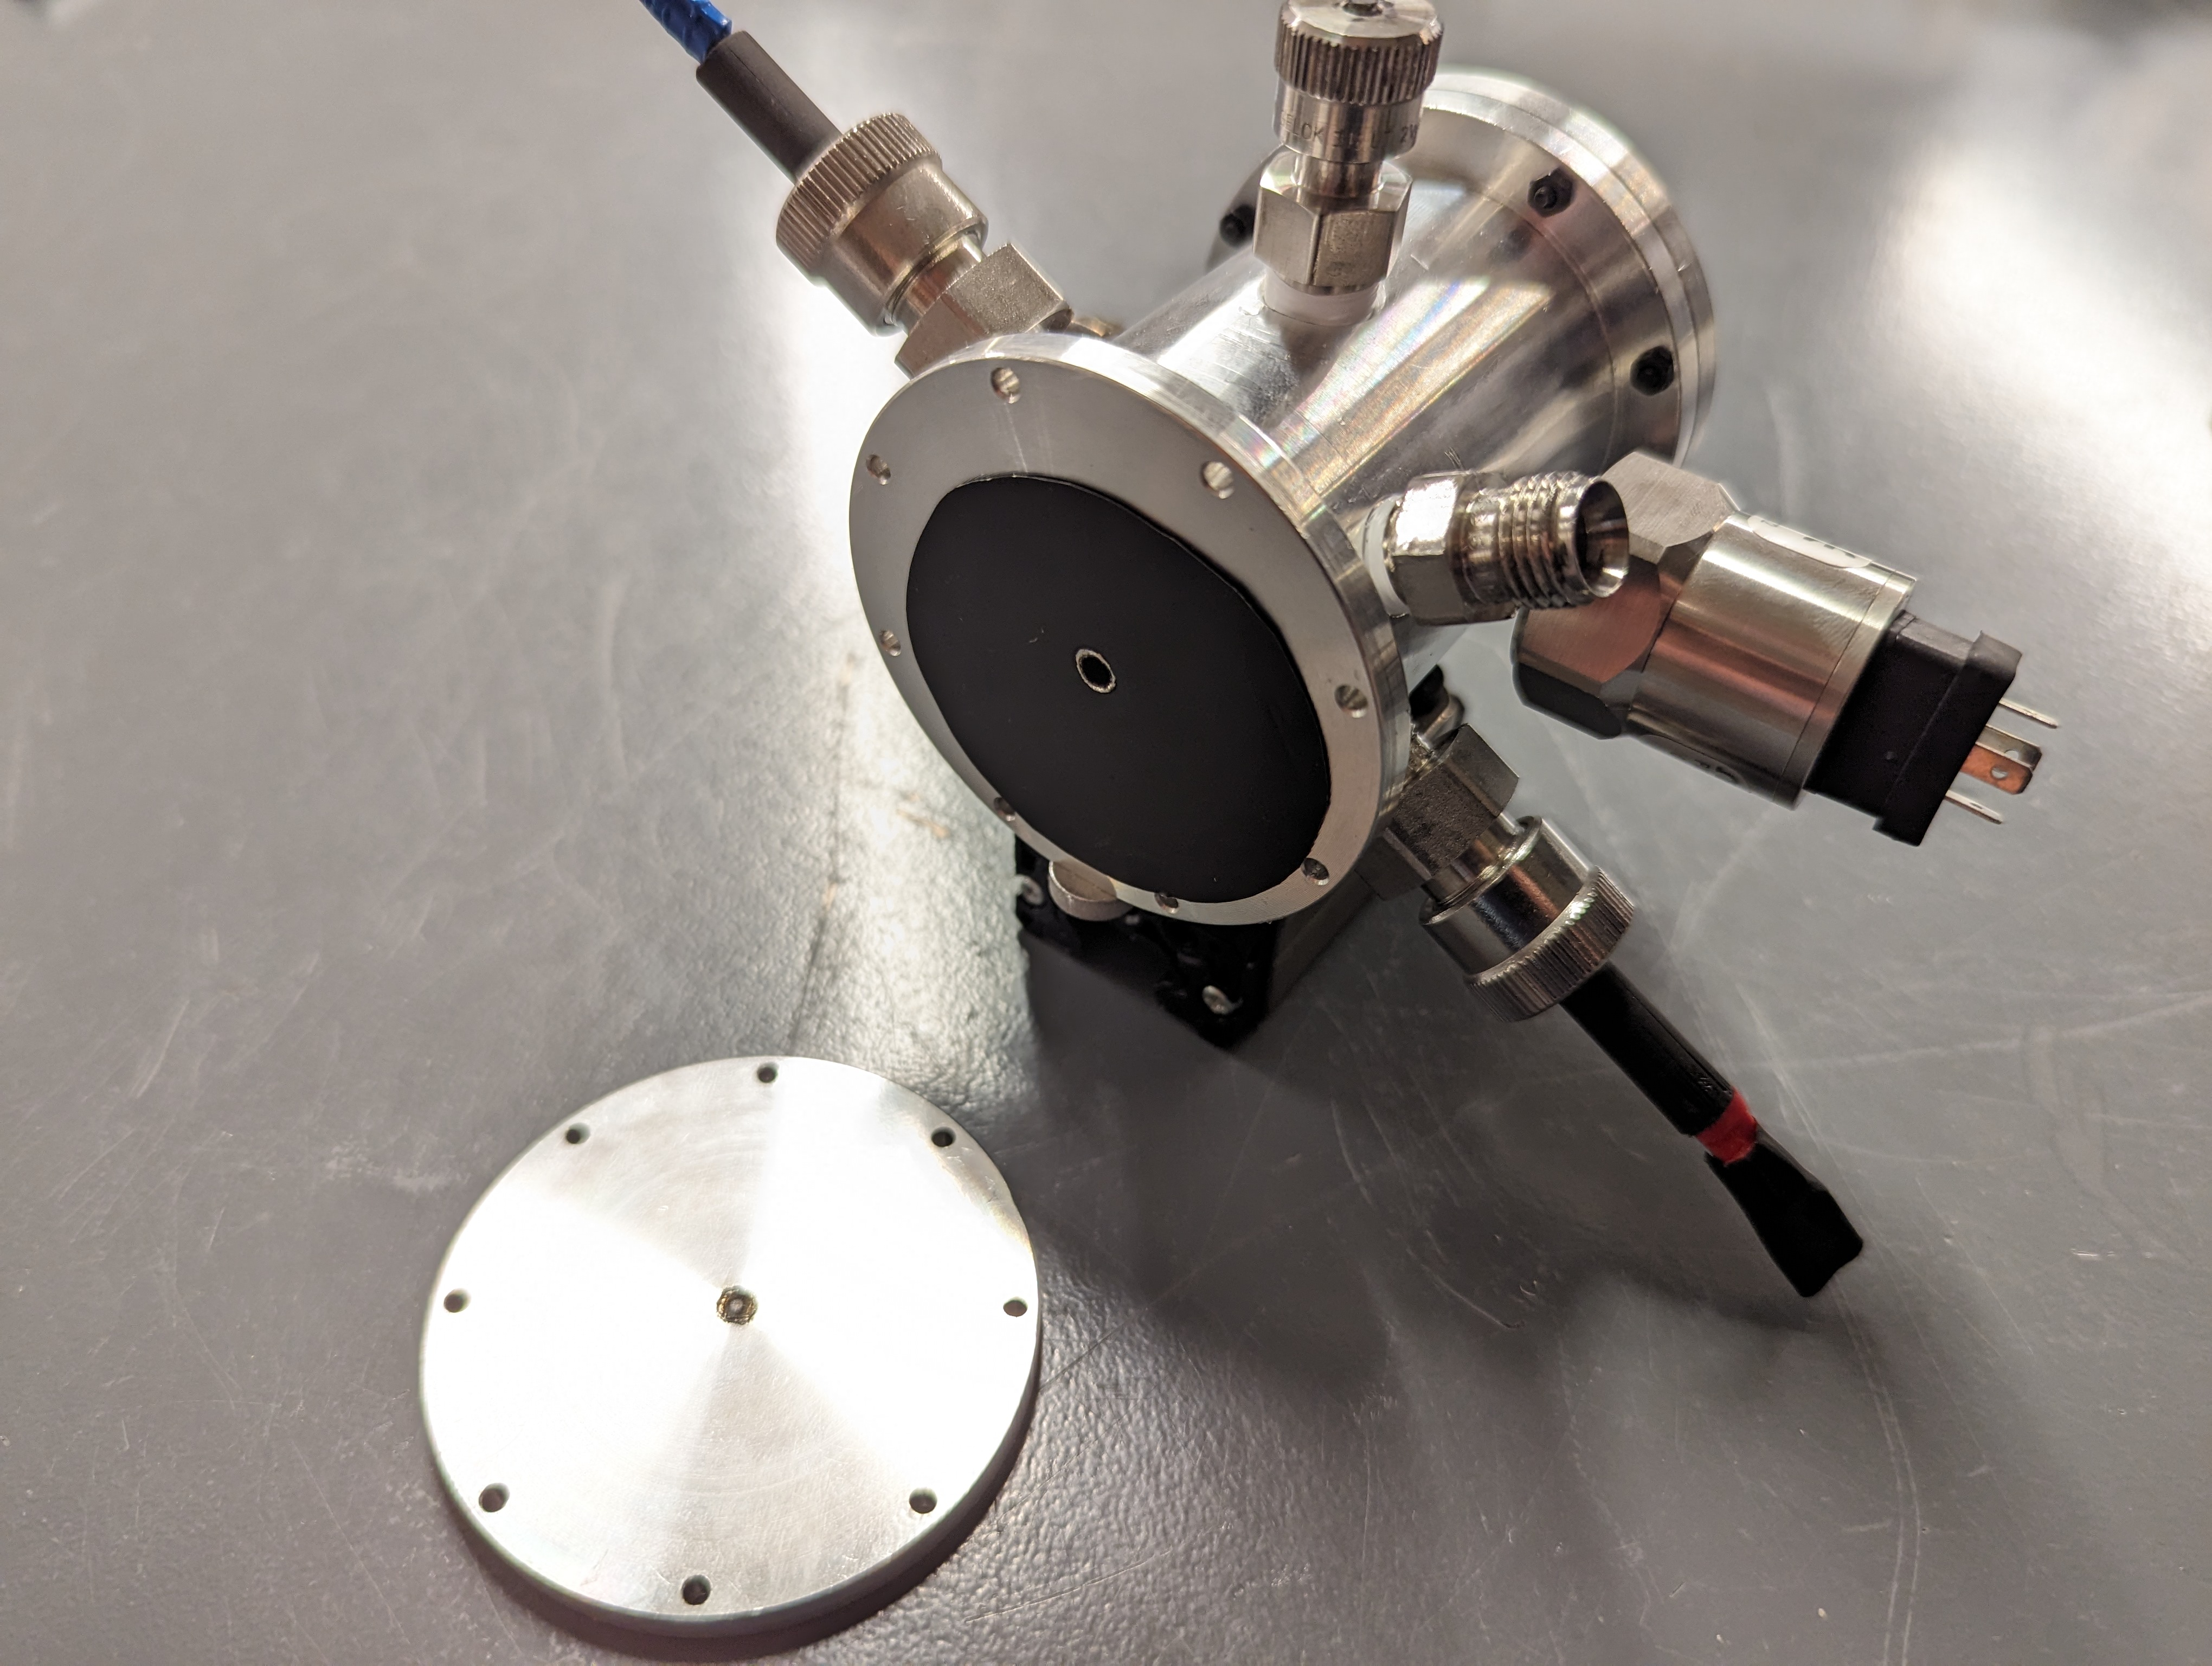
\includegraphics[width=0.75\textwidth]{assets/4 experiments/V2 test damage.jpg}
            \caption{Damage to the flat rear plate of the thruster after two \qty{3}{kW} laser shots. The black sheet is laser-absorbing ADD PART NUMBER aluminum foil, used in a failed attempt to protect the rear plate from damage.}
        \end{figure}

        \subsubsection{Window extension tube - discussion}
        
        After the first CW LSP, more CW and pulsed shots were attempted. These continued to damage the rear window. Eventually, a \qty{3}{s} CW shot melted it severely enough that 

        \begin{figure}[!ht]
            \centering
            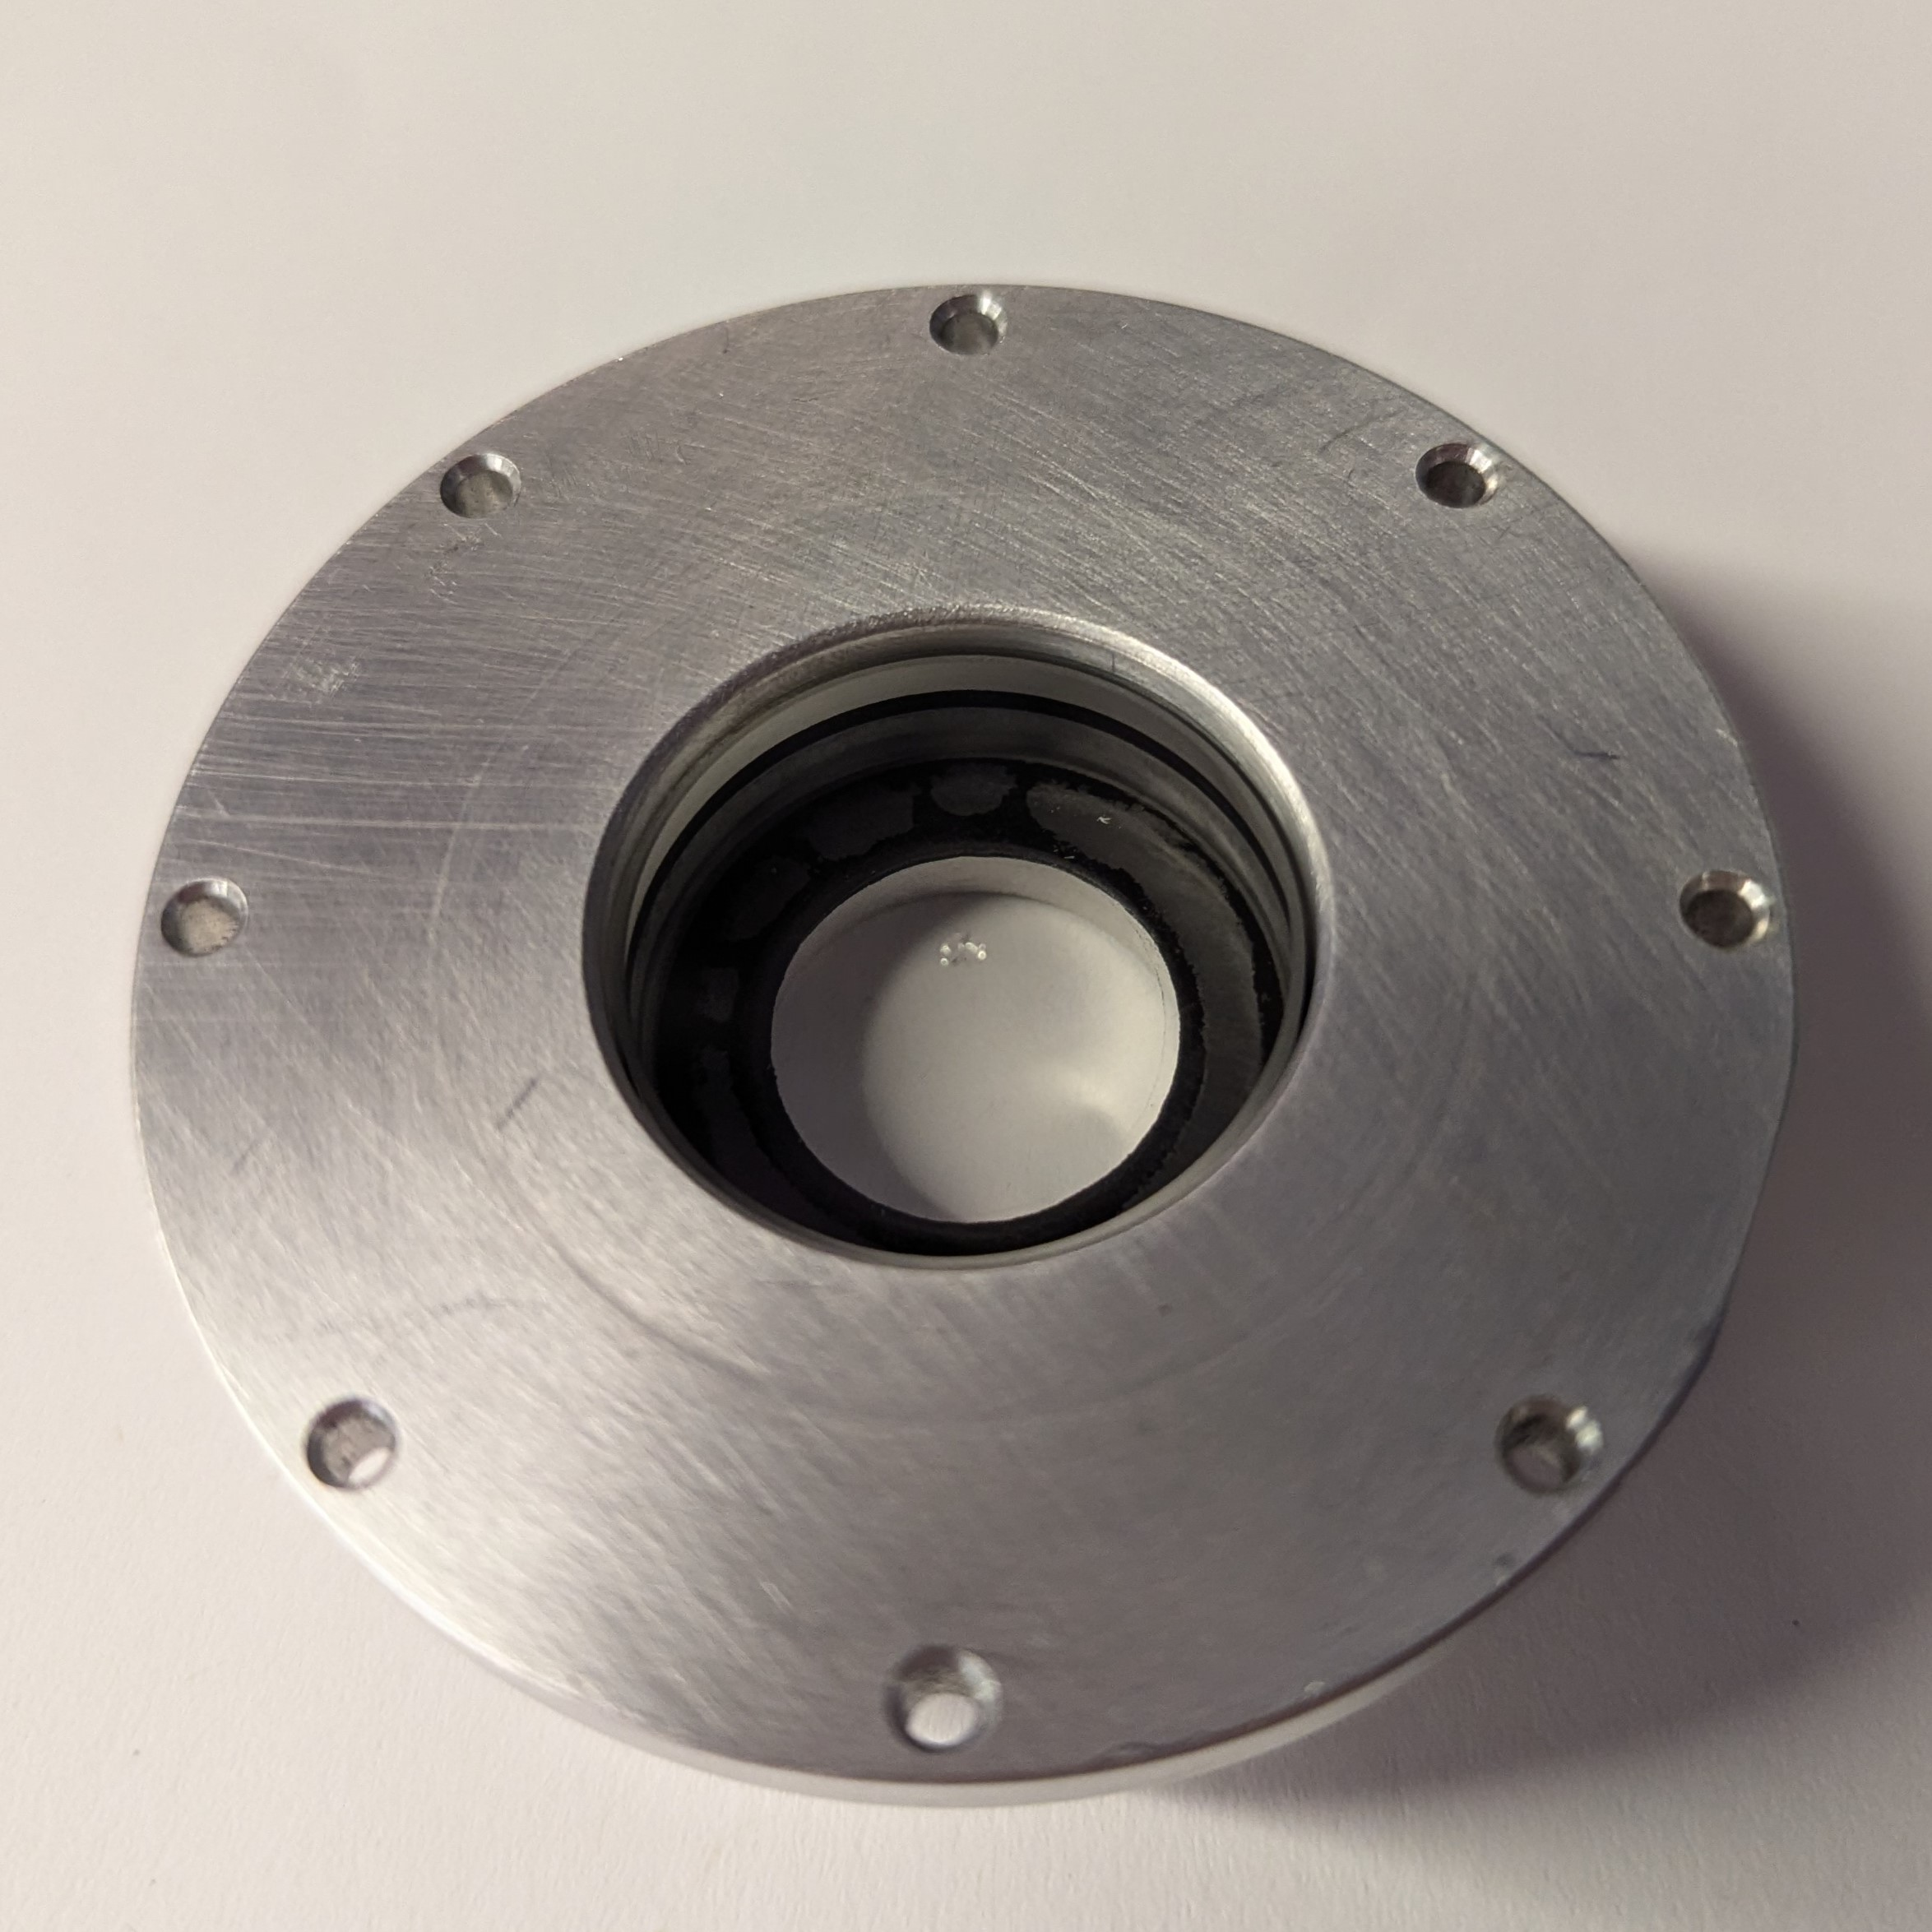
\includegraphics[width=0.5\textwidth]{assets/4 experiments/window damage.jpg}
            \caption{Rear window damage on V2}
        \end{figure}

        The solution chosen was to manufacture a window extension tube, moving the rear window downstream to where the laser flux density is comparable to the front window, where no damage was seen.

        [drawing of extension tube, calculations of laser flux]

\section{Cold flow thrust tests}

    \subsection{Cold flow test friction HYSTERESIS}

        [FRICTION HYSTERESIS PROBLEMS: TO DISCUSSION] To correct these problems, a more sensitive load cell was installed with a \qtyrange{0}{5}{N} force sensing range (Honeywell FSG005WNPB). Lubricant was also added to the cart's bearings. However, the issue remained.

        Here are some results of the cold flow tests with the new load cell. Here, I did multiple firings with a 200g preload. We didn't calibrate the load cell, as we just want to look at hysteresis. What we see is that sometimes the final thrust is higher than the initial thrust, sometimes it's the other way around. According to me, this is due to the friction in the rail stopping the thruster from resetting at the same place every time. When we get to doing thrust tests with LSP, we'll do a few and average them. At least the initial increase looks fairly repeatable.
        Going forward, I think the only way to get really nice thrust data would be to use a rotating arm thrust stand. To be done after I finish the thesis! \todo{edit this to read more academic}

        \begin{figure}[h]
            \centering
            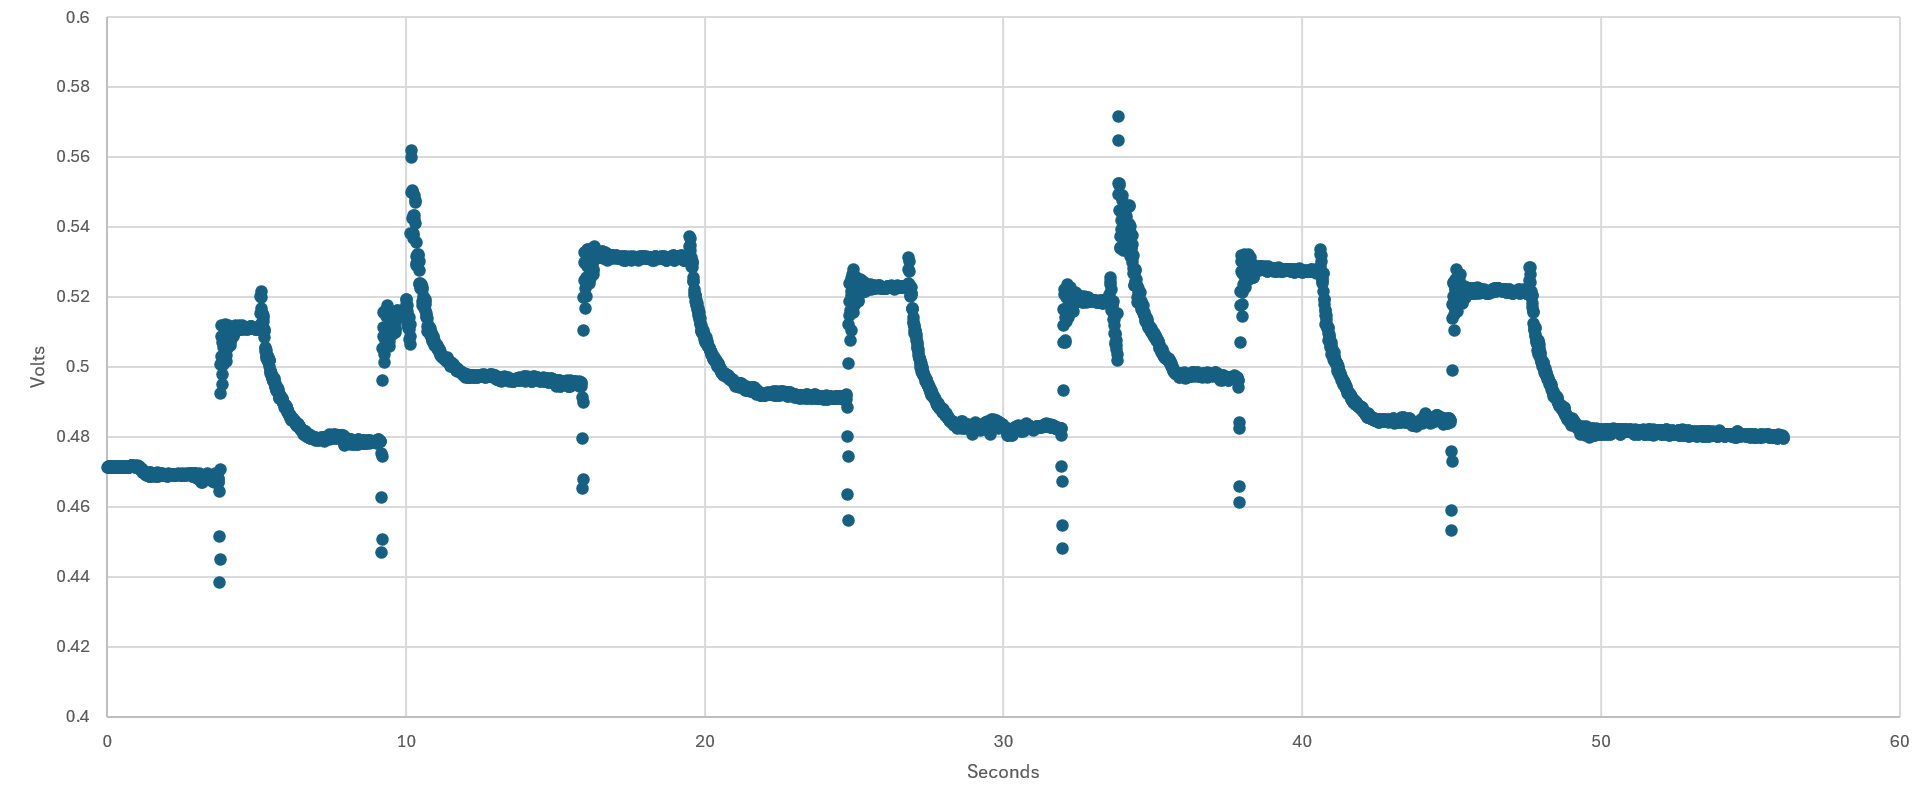
\includegraphics[width=0.8\linewidth]{assets/5 discussion/hysterisis.png}
            \caption{PLACEHOLDER HYSTERESIS GRAPH}
            \label{fig:double choke sizing}
        \end{figure}

        \todo{make graph better, not excel and calibrate}

        The discontinuities at 10 and 35 seconds are due to me accidentally shutting off the gas supply.

        The present type of thrust stand is therefore inadequate for future thrust tests. A different type of thrust stand (e.g. a rotating arm), should be built to measure thrust in a repeatable manner.

    \subsection{Effective throat area - discussion}
            
        With the cold flow thrust tests completed, the effective throat area, $A^*$, was determined to be \qty{3.46e-8}{m^2}, or a diameter of \qty{0.21}{mm}. Although the throat was physically measured to be \qty{0.8}{mm} in diameter (a 20G pin could pass through it), boundary layer effects at this size greatly reduce the effective throat area.

        Indeed, the effective

        [Add Reynolds number at throat? -> calculation]

        [ADD SAAD BLOWDOWN DISCUSSION]

        [CITE 2 ASME STUDIES]

    \subsection*{Other stuff}

\section{Flowing QCW LSP discussion}

    \subsection{New nozzle design}

    Attempts at pulsed LSP initiation with the original nozzle gave 

    \begin{figure}[!ht]
        \centering
        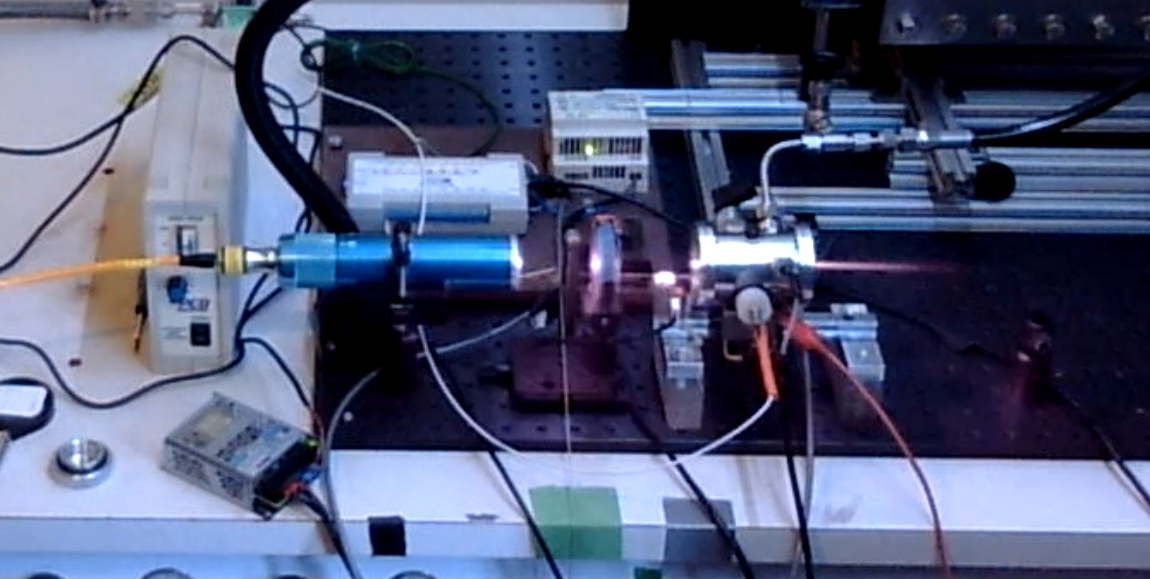
\includegraphics[width=0.5\textwidth]{assets/5 discussion/Nozzle ablation.png}
        \caption{Nozzle ablation during flowing test}
        \label{fig:nozzle ablation}
    \end{figure}

    \autoref{fig:nozzle ablation} shows nozzle ablation during a QCW flowing test. No LSP was initiated, however a plasma trail can be seen exiting the nozzle. This plasma was generated by nozzle ablation, proving that this experiment can operate as a laser ablation thruster. This unfortunately not what the thruster was designed for. \todo{Looking at the video from the last shot (no electrodes, so no LSP), we do have a plasma-powered rocket engine!  It's just that it's an ablation plasma, not the kind we want}

    \textcite{toyodaThrustPerformanceCW2002} uses a refractory metal, tungsten, as the nozzle material. Other possibilites were: machinable cermaics (expensive on McMaster!), stainless steel. Graphite was chosen because it is already used for model rockets and is economical. However, it is messy when you machine it \todo{Refer to lit review article when talk about graphite nozzle, which study we base ourself on to choose a graphite nozzle}

    \begin{figure}[!ht]
        \centering
        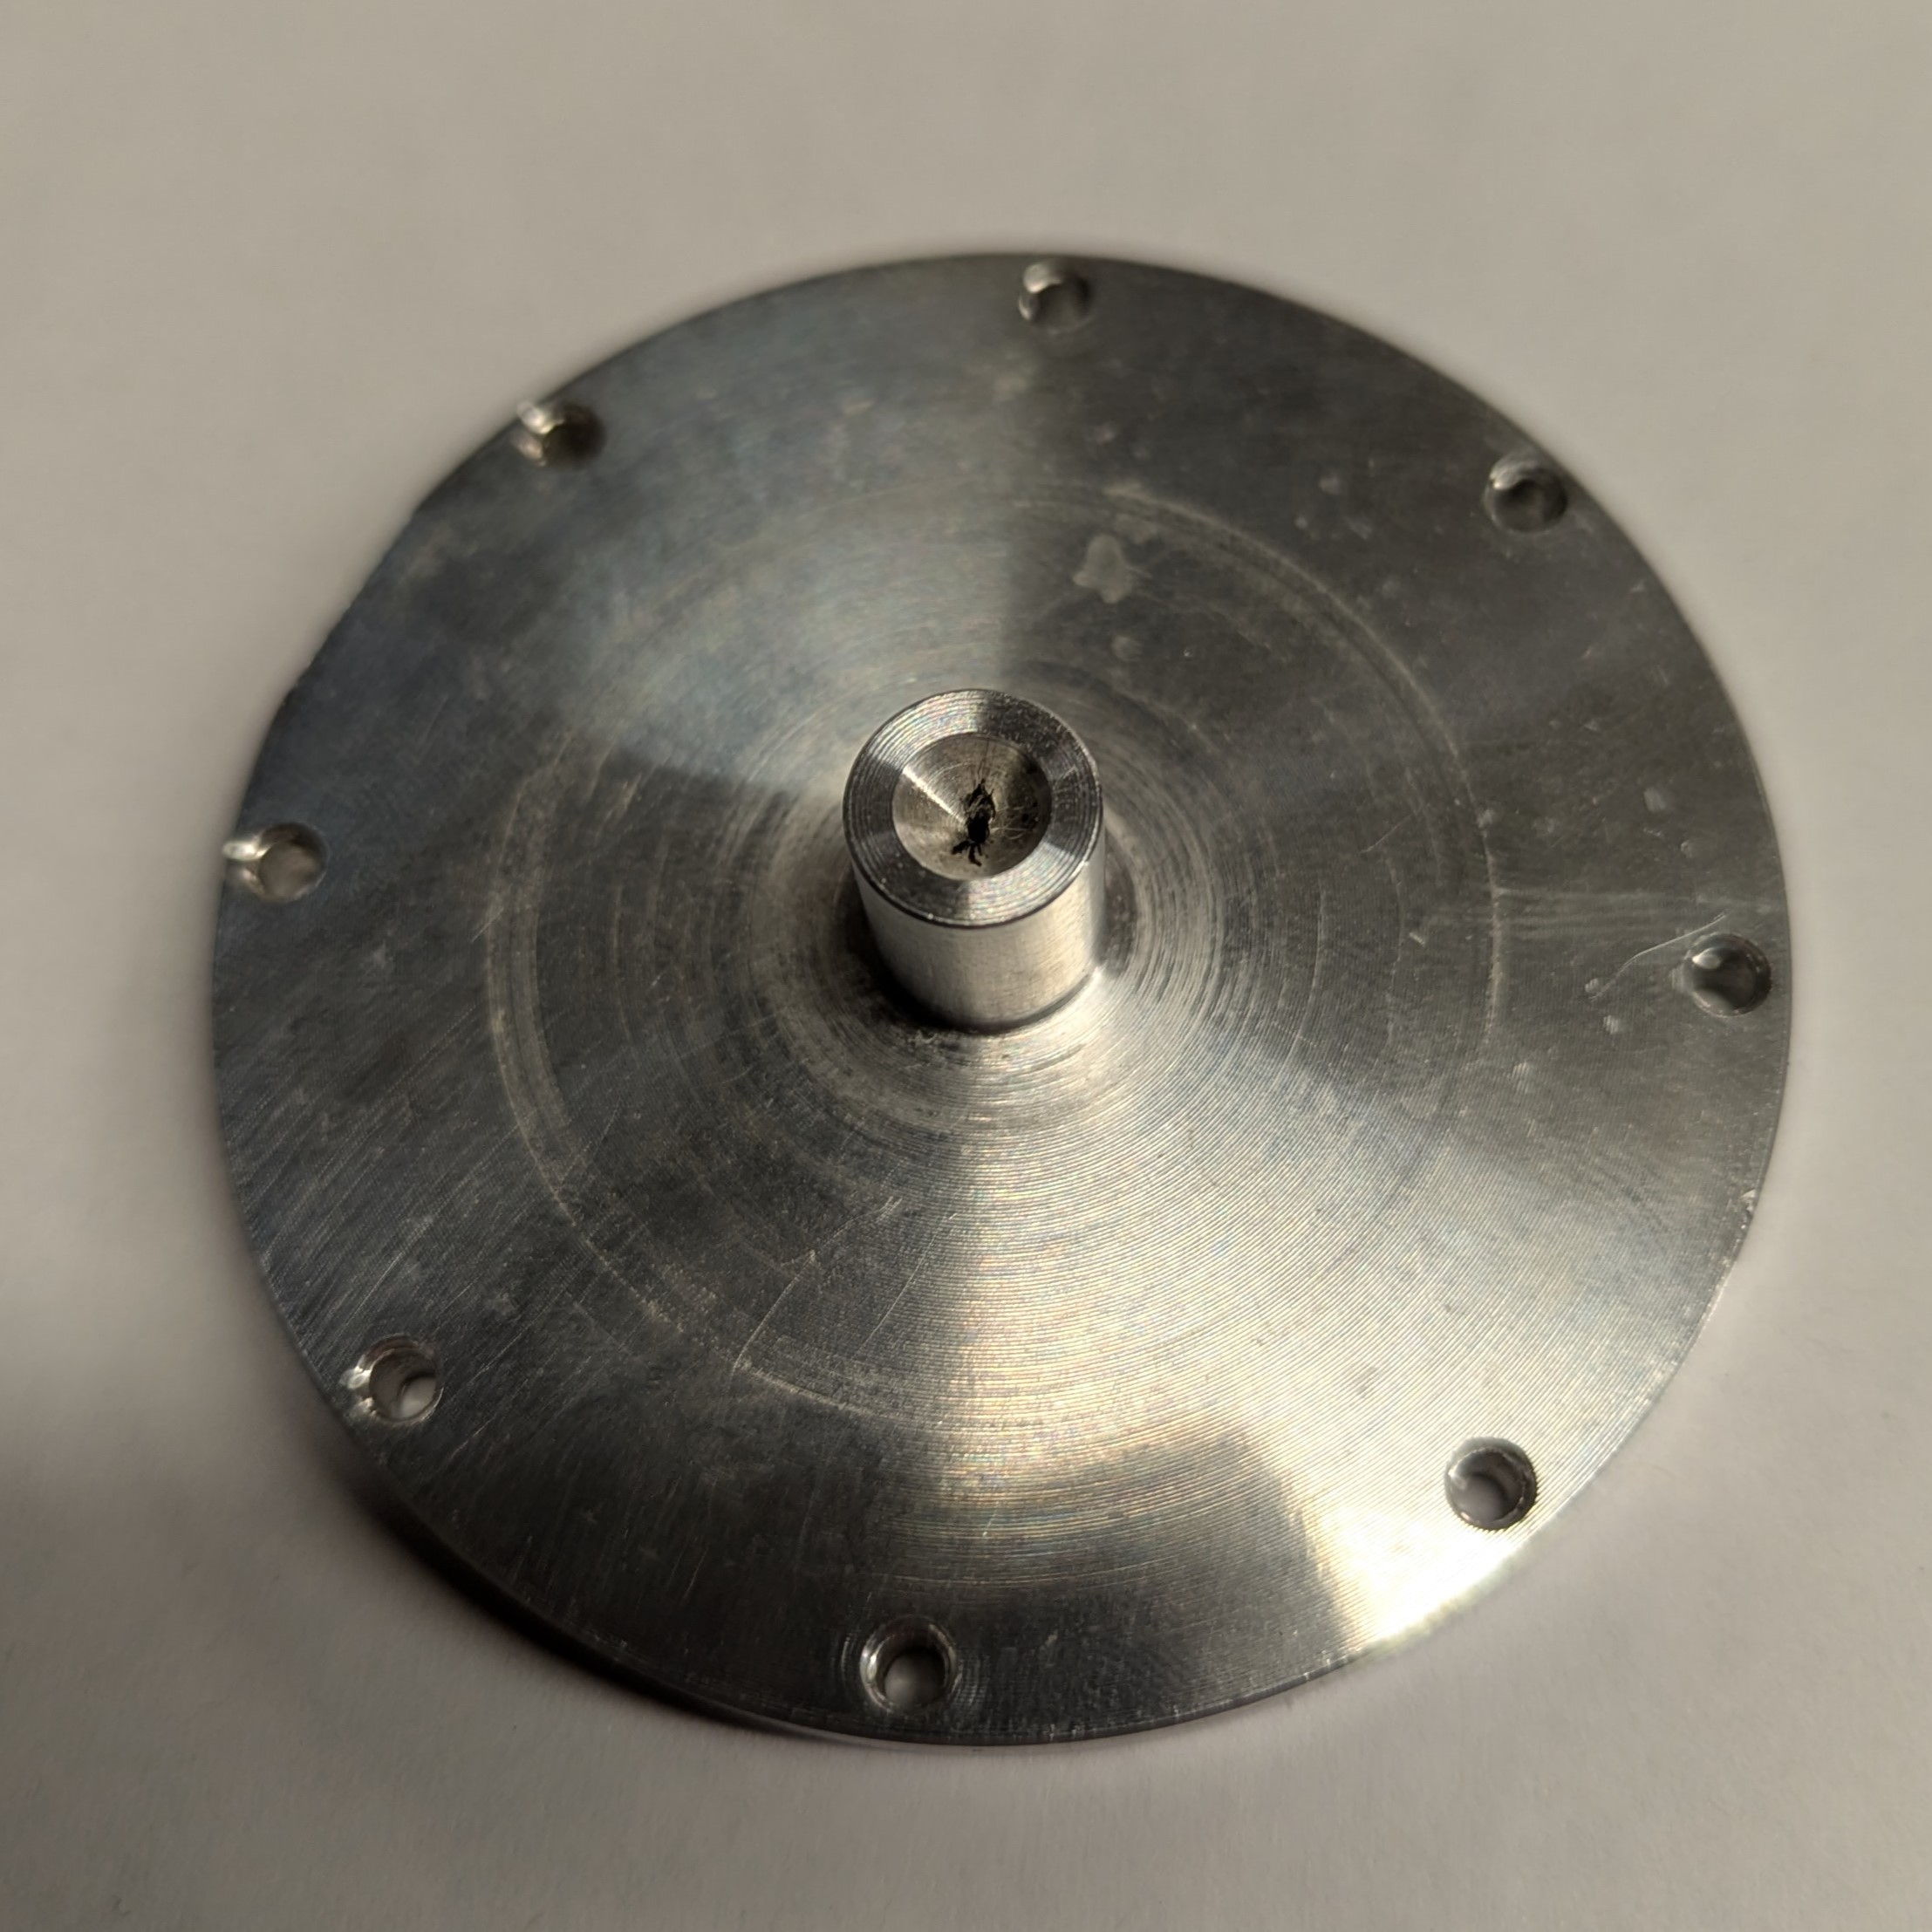
\includegraphics[width=0.5\textwidth]{assets/4 experiments/Nozzle damage.jpg}
        \caption{Nozzle laser damage}
    \end{figure}

    To solve the ablation of the aluminum nozzle under pulsed laser shots, the V2 thruster inner cylinder was modified, and a new backplate was manufactured to accept graphite nozzle inserts. These inexpensive, changeable inserts are made from superfine iso-molded graphite rods sourced from Graphitestore (0.500" diameter x 12"L, SKU GT001685).

    [image of drawing highlighting changes to inner cylinder], other parts that were made.

% New parts that were made and why?
    % Nozzle/retaining plate
    % Window extension
    %  NPT fitting to calculate m_dot in bubble meter
Due to machining delays however, these final parts were not tested. 

% Future work:
% - Validate that window extension works
% - Characterize nozzle throat effective diameter

    